\documentclass[10pt, compress]{beamer}

\usetheme{metropolis}
\usepackage{appendixnumberbeamer}

\usepackage{tikz-dependency}
\usepackage{caption}
\usepackage{polyglossia}
\usepackage{booktabs}
\usepackage{tabularx}
\usepackage{alltt}
\usepackage[scale=2]{ccicons}

\usepackage{pgfplots}
\usepgfplotslibrary{dateplot}

\usepackage{xspace}
\newcommand{\themename}{\textbf{\textsc{metropolis}}\xspace}

% commands from the paper
%\setmainfont[Scale=1.0]{Fira Sans Light}

\newfontfamily\gtfont[Scale=1.1,Letters=SmallCaps]{Linux Libertine O}
\newcommand{\udtag}[1]{{\ll \textsc{#1}}}
\newcommand{\gtlabel}[1]{{\gtfont #1}}
\newcommand{\udlabel}[1]{{\tt #1}}
\newfontfamily\udfont[Scale=0.9,Letters=SmallCaps]{Linux Libertine O}
\newcommand{\utag}[1]{{\udfont#1}}
\newcommand{\ufeat}[1]{{\udfont#1}}
\newcommand{\tgl}[1]{{\em #1}}
\setmonofont[Scale=MatchLowercase]{DejaVu Sans Mono}

% commands from the paper


\newcommand{\myarrow}[1][-45]{%
  \mathrel{%
    \text{$
     \begin{tikzpicture}[baseline = -0.5ex]
       \node[inner sep=0pt,outer sep=0pt,rotate = #1] (a) at (0,0)  {$\xrightarrow{}$};
    \end{tikzpicture}
    $}%
  }%
}%




\title{Class 05: Named-entity recognition}

\begin{document}

\maketitle

\begin{frame}{Information extraction}


\end{frame}


\begin{frame}{Named-entity recognition}


\end{frame}

\begin{frame}{Named-entity types}


\end{frame}

\begin{frame}{Ambiguity}

\end{frame}


\begin{frame}{Sequence labelling}


\end{frame}

\begin{frame}{Example}

\end{frame}


\begin{frame}{Typical features}

\end{frame}


\begin{frame}{Gazetteers}


\end{frame}

\begin{frame}{Domains}


\end{frame}


\begin{frame}{Evaluation}


\end{frame}

\begin{frame}{Producing training data}


\end{frame}

\begin{frame}{Manually annotated}


\end{frame}

\begin{frame}{Wikipedia/1}
% also manually annotated, kindof

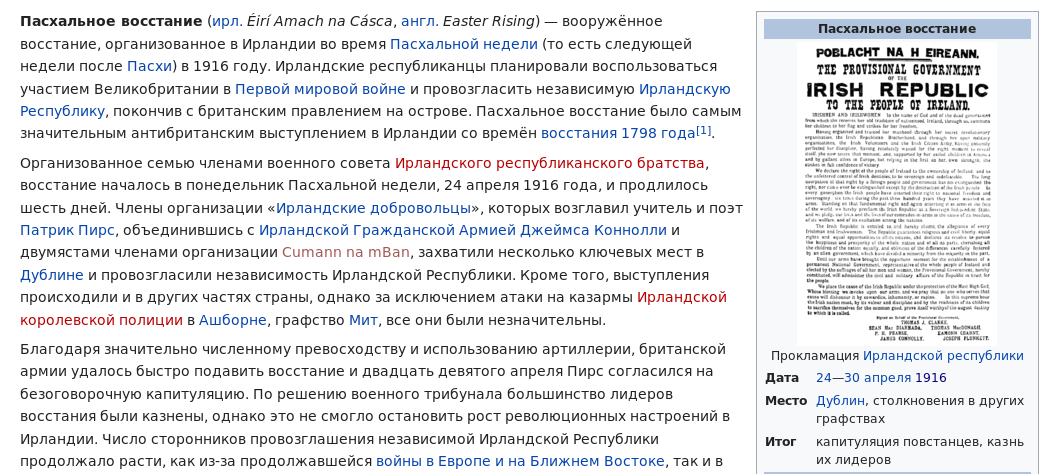
\includegraphics[width=\textwidth]{graphics/wikipedia-1.png}

\end{frame}

\begin{frame}{Wikipedia/2}

{\tt
Члены организации «[[Ирландские добровольцы]]», которых возглавил учитель 
и поэт [[Пирс, Патрик|Патрик Пирс]], объединившись с [[Ирландская гражданская армия|Ирландской Гражданской Армией]] [[Коннолли, Джеймс|Джеймса Коннолли]] и двумястами членами организации [[Совет ирландских женщин|Cumann na mBan]], захватили несколько ключевых мест в [[Дублин]]е и провозгласили независимость Ирландской Республики. 
}
\end{frame}

\begin{frame}{Wikipedia/3}
 % Cats

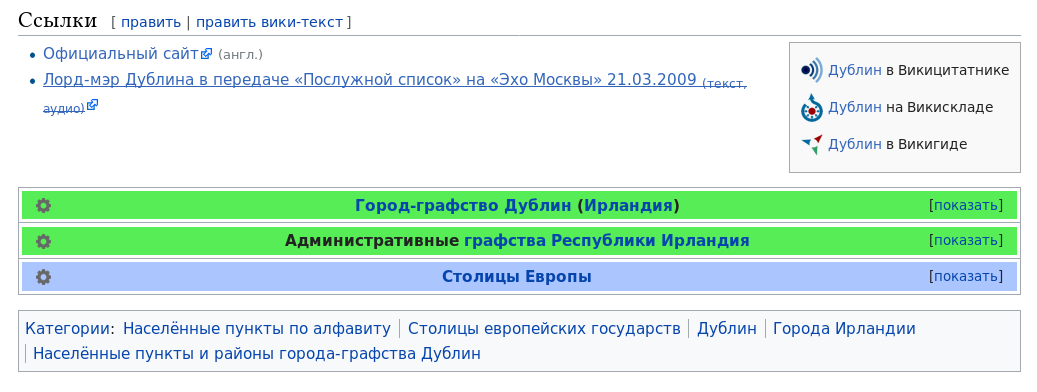
\includegraphics[width=\textwidth]{graphics/wikipedia-2.png}

\end{frame}

\begin{frame}{Wikipedia/4}

% Ирландские добровольцы
% Пирс, Патрик
% Ирландская гражданская армия
% Коннолли, Джеймс
% Совет ирландских женщин
% Дублин

\end{frame}

\begin{frame}{Wikipedia/5}

{\tt
Члены организации «[{\sc ORG} Ирландские добровольцы]», которых возглавил 
учитель и поэт [{\sc PER} Патрик Пирс], объединившись с [{\sc ORG} Ирландской 
Гражданской Армией] [{\sc PER} Джеймса Коннолли] и двумястами членами 
организации \alert<2>{Cumann na mBan}, захватили несколько ключевых мест 
в [{\sc LOC} Дублине] и провозгласили независимость \alert<2>{Ирландской Республики}.
}

\end{frame}

\begin{frame}{Wikipedia/6}

\begin{itemize}
  \item Nothman, J. (2008) ``Transforming Wikipedia into Named Entity Training Data''. \emph{Proceedings of the Australasian Language Technology Association Workshop}
  \item Hahm, Y. et al. (2014) ``Named Entity Corpus Construction using Wikipedia and DBpedia Ontology''. \emph{LREC 2014}
  \item Сысоев, А. А. and Андрианов, И. А. (2016) ``Named entity recognition in Russian: The power of a Wiki-based approach''. \emph{Proceedings of the International Conference “Dialogue 2016”}
\end{itemize}

\end{frame}



\begin{frame}[standout]
Shared tasks
\end{frame}

\begin{frame}{CoNLL 2003}


\end{frame}

\begin{frame}{FactRuEval 2016}


\end{frame}

\begin{frame}{First track}

\end{frame}


\begin{frame}{Layered annotation model}


\end{frame}

\begin{frame}{Data}

\end{frame}

\begin{frame}{Participants}

\end{frame}

\begin{frame}{Results}

\end{frame}

\begin{frame}[standout]
Practical
\end{frame}




\end{document}
